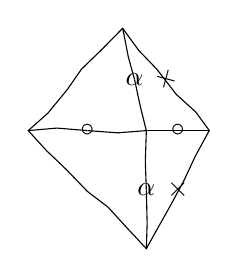
\begin{tikzpicture}[rotate=0,every node/.style={scale=1}]

\tikzstyle{MainLevee}=[decorate,decoration={random steps,amplitude=1pt,segment length=10pt}]

\coordinate (A) at (0,0);
\coordinate (B) at (1.2,1.3);
\coordinate (C) at (2.3,0);
\coordinate (D) at (1.5,-1.5);
\coordinate (O) at (1.5,0); %le centre du losange

%%%%%Les marques d'égalité de longueurs sur les diagonales :
\coordinate (A') at (0.75,0); %le milieu de la diagonale [AO]
\coordinate (B') at (1.35,0.65);
\coordinate (C') at (1.9,0);
\coordinate (D') at (1.5,-0.75);
\node at (A'){$\circ$};
\node at (B'){$\alpha$};
\node at (C'){$\circ$};
\node at (D'){$\alpha$};
%%% Les marques d'égalité de longueurs sur 2 côtés
\draw (1.75,0.65) node[rotate=30] {$\times$};
\draw (1.9,-0.75) node[rotate=0] {$\times$};

\draw[MainLevee] (A) -- (B) -- (C) -- (D) --cycle;

\draw[MainLevee] (A)--(A'); 
\draw[MainLevee] (A')--(O);
\draw[MainLevee] (B)--(B'); 
\draw[MainLevee] (B')--(O);
\draw[MainLevee] (C)--(C'); 
\draw[MainLevee] (C')--(O);
\draw[MainLevee] (D)--(D'); 
\draw[MainLevee] (D')--(O);

\end{tikzpicture}